\documentclass{sintefbeamer}

% packages, font, color, and newcommands
\usepackage{amsfonts, amsmath, oldgerm, lmodern, bm}
% \usepackage[font={footnotesize}]{caption}
\usepackage{natbib}
\usepackage{url}
\usepackage{tikz}
\usepackage{amssymb}
\usepackage{amsmath}
\usepackage{amsthm}
\usepackage{mathrsfs}
\usepackage{empheq}
\usepackage{mdframed}
\usepackage{bm}
\usepackage{animate}
\usepackage{xcolor,colortbl}
\usepackage{graphicx}
\bibliographystyle{apalike}
\usefonttheme{serif}
\usetikzlibrary{calc}
\definecolor{carminered}{rgb}{1.0, 0.0, 0.22}
\definecolor{burgundy}{rgb}{0.5, 0.0, 0.13}
\title{Energy budget for disperse two-phase flow made of fluid inclusions}
\subtitle{An hybrid model approach}
\author{\href{http://basilisk.fr/sandbox/fintzin/Rising-Suspenion/RS.c}{\underline{N. Fintzi}\footnote{IFP \'Energies Nouvelles, France}$^{,2}$}, JL. Pierson$^1$ and D. Lhuillier\footnote{Sorbonne Universit\'e, France}}
% \date{Created on May 22, 2022}
\definecolor{burntorange}{rgb}{0.8, 0.33, 0.0}
\titlebackground{image/HOMOGENEOUS_NEW/P_PHI_5_l_1_Ga_100.png}

% document body
\addtobeamertemplate{navigation symbols}{}{%
    \usebeamerfont{footline}%
    \usebeamercolor[fg]{footline}%
    % \hspace{1em}%
    % \vspace{1em}%
    \insertframenumber/\inserttotalframenumber
}
\usepackage{stmaryrd}


\begin{document}
\maketitle
\section*{}
\section*{}

\begin{frame}
  \frametitle{Objectives}

  \begin{enumerate}
    \item Deriving the averaged \textbf{pseudo turbulent} energy equations for dispersed two-phase flow made of fluid particles. 
    \begin{itemize}
      \item The dispersed phase is averaged using a kinetic theory-like approach \citep{jackson1997locally,zhang1994averaged}
      \item The fluid phase is averaged following the classic average method \citep{drew1983mathematical}. 
    \end{itemize}
    \item Discus the influence of the droplets internal motion on the \textbf{pseudo turbulent} energy equations. 
    \begin{itemize}
      \item In the dilute limit, the droplet internal motions can be represented as a linear, quadratic or cubic function of the distance to the center of mass leading to important simplifications.
    \end{itemize}
    \item Derive a first approximation of the \textbf{particle-particle stress} in the low capillary number regime. 
    \begin{itemize}
      \item We model the particle-particle contact force with the capillary pressure. 
    \end{itemize}
  \end{enumerate}
\end{frame}
\section{Local scale energy equations}
\section*{}

\begin{frame}
  \frametitle{Problem statement}

  \begin{figure}[h!]
    \centering
    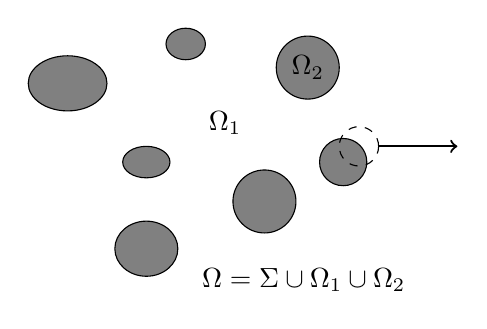
\begin{tikzpicture}
        \foreach \x/\y/\ra/\r in {
        1/3/0.2/0.25,
        2.55/2.7/0.4/0.4,
        0.5/0.4/0.35/0.4,
        2/1/0.4/0.4,
        3/1.5/0.3/0.3,
        0.5/1.5/0.2/0.3,
        -0.5/2.5/0.35/0.5}{
            \draw[fill=gray](\x,\y) ellipse(\r cm and \ra cm);
        }
        \draw[dashed](3.2,1.7)circle(0.25);
        % \draw[thick,->](3.2,1.7)++(0.1767,0.1767)--++(0.4,0.4)--++(1,0);
        \draw[thick,->](3.2,1.7)++(0.25,0)--++(1,0);
        \draw(2.55,2.7)node{$\Omega_2$};
        \draw(1.5,2)node{$\Omega_1$};
        \draw(2.5,0)node{$\Omega = \Sigma \cup \Omega_1 \cup \Omega_2$};
        % \draw(2.5,-1)node{$\Sigma = \sum_\alpha \Sigma_\alpha$};
        % \draw(2.5,-0.5)node{$\Omega_2 = \sum_\alpha \Omega_\alpha$};
    \end{tikzpicture}
    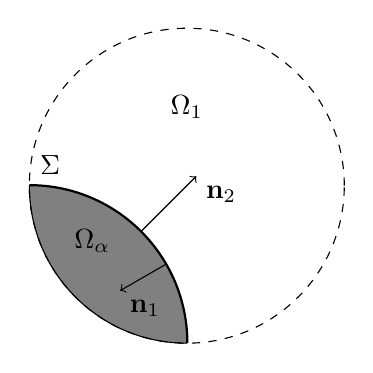
\begin{tikzpicture}%[scale = 0.9]
        \draw[very thick](0:2)arc(0:90:2)node[above right]{$\Sigma$};
        \draw[fill=gray](0:2)arc(0:90:2)arc(180:270:2);
        \draw[dashed](2,2)circle(2);
        \draw[->](1.42,1.42)--++(0.7,0.7)node[below right]{$\textbf{n}_2$};
        \draw[->](1.73,1)--++(-0.577,-0.333)node[below right]{$\textbf{n}_1$};
        \draw(2,3)node{$\Omega_1$};
        \draw(0.8,1.3)node{$\Omega_\alpha$};
    \end{tikzpicture}
    \caption{Domain definitions and scheme of the topology of dispersed two-phase flows.}
    \label{fig:Scheme}
\end{figure}

The phase and interface indicator functions : 
\begin{align}
  \chi_k(\textbf{x},t) &=  \left\{
    \begin{tabular}{cc}
      $1 \;\text{if} \;\textbf{x} \in \Omega_k(t)$\\
      $0 \;\text{if} \;\textbf{x} \notin \Omega_k(t)$
    \end{tabular}
    \right.
    % \text{for $k = 1,2$},
    % \label{eq:PIF}
    &&
  \delta_I(\textbf{x},t) &=  \left\{
    \begin{tabular}{cc}
      $1 \;\text{if} \;\textbf{x} \in \Sigma(t)$\\
      $0 \;\text{if} \;\textbf{x} \notin \Sigma(t)$
    \end{tabular}
    \right.,
    \label{eq:PIF_I}
\end{align}

\end{frame}

  \begin{frame}
    \frametitle{Local scale energy balance.}
    The total energy $E_k^0 = e_k^0 + u^0_k /2$ of phase $k$ follows :
  \begin{equation}
    \pddt (\rho_kE_k^0)  
    + \div (
        \rho_kE_k^0\textbf{u}_k^0
        + \textbf{q}_k^0
        - \textbf{u}_k^0 \cdot \bm{\sigma}_k^0 
        )
    = 
    \textbf{u}_k^0 \cdot \textbf{b}_k^0
    \ \ \ \ 
    \text{in} 
    \ \ \ \ 
    \Omega_k(t)
  \end{equation}
  And at the interface : 
  \begin{align}
    \label{eq:dt_rhoI_uI2}
    \Jump{\textbf{u}_k^0 \cdot \bm{\sigma}_k^0}
    &= 
     \gamma\kappa\textbf{n}\cdot \textbf{u}_{I}^0\\
    \label{eq:dt_rhoIe_I}
    \Jump{ \textbf{q}_k^0}
    &= 
     0
\end{align}
    \begin{itemize}
      \item The superscript $^0$ indicated that it is a local quantity.
      \item $\rho_k$  density of phase $k$. 
      \item $\textbf{q}_k^0$  heat flux.
      \item $\textbf{u}_k$  Velocity of phase $k$.
      \item $\textbf{b}_k^0 = \rho_k \textbf{g}$  local body force.  
      \item $\gamma$ and $\kappa$  surface tension coefficient and curvature of the surface.  
      \item $e_k^0$  local internal energy. 
    \end{itemize}
  
  \end{frame}
  \begin{frame}
    \frametitle{Total energy of a single fluid particle}
    We define the total volume and surface energy of the particle $\alpha$ by, 
    \begin{align*}
      m_\alpha E_\alpha(t) 
   = \int_{\Omega_\alpha(t)} \rho_2 [e_2^0 + (u_2^0)^2/2] d\Omega,
    &&
    s_\alpha(t) E_{I\alpha}(t) 
    = \int_{\Sigma_\alpha(t)} \gamma d\Sigma,\\
    = m_\alpha e_\alpha 
    + W_\alpha
    + m_\alpha (u_\alpha)^2/2
  \end{align*}

  \begin{itemize}
    \item $e_\alpha =  \int_{\Omega_\alpha(t)} \rho_2 e_2^0 d\Omega$ internal energy of the particle. 
    \item $W_\alpha = \int_{\Omega_\alpha(t)} \rho_2 (w_2^0)^2 d\Omega$ internal kinetic energy of the particle. 
    \item $\textbf{u}_\alpha$ particle's center of mass velocity. 
    \item $\textbf{w}_2^0 = \textbf{u}_2^0 - \textbf{u}_\alpha$ velocity internal particle velocity fluctuation. 
    \item $ m_\alpha (u_\alpha)^2/2$ center of mass kinetic energy of the particle. 
  \end{itemize}

  \textcolor{red}{\textbf{Warning : } In the next slides we use the notations :  $\intO{\ldots} = \int_{\Omega_\alpha} \dots d\Omega$ and  $\intS{\ldots} = \int_{\Sigma_\alpha} \dots d\Sigma$.}
\end{frame}

\begin{frame}
  \frametitle{Lagrangian balance for a single fluid particle ? }
  We first take the Lagrangian derivative $E_\alpha$ : 
  \begin{multline*}
    \ddt \int_{\Omega_\alpha(t)} \rho_2 E_2^0 d\Omega
    = \intO{ \pddt (\rho_2 E_2^0) + \div\left(\rho_2 E_2^0\textbf{u}_2^0\right) }
    + \underbrace{\intS{ \rho_2 E_2^0 (\textbf{u}_I^0-\textbf{u}_2^0)\cdot \textbf{n}_2 }}_\text{Mass transfer term}.
  \end{multline*}
  \begin{equation*}
    \ddt s_\alpha\gamma
    = \intS{\Jump{\textbf{u}_k\cdot \bm\sigma_k^0}}
  \end{equation*}
  Using the volume and surface local energy conservation equations gives,  
  \begin{align}
    \ddt (m_\alpha E_\alpha + s_\alpha \gamma)
    &= 
    m_\alpha \textbf{u}_\alpha \cdot \textbf{g}
    +\textbf{u}_\alpha \cdot \intS{\bm{\sigma}_1^0 \cdot \textbf{n}_2}   
    +\intS{\textbf{w}_1^0 \cdot \bm{\sigma}_1^0 \cdot  \textbf{n}_2} 
    - \intS{\textbf{q}_1^0 \cdot \textbf{n}_2}
  \end{align}
\begin{itemize}
  \item $m_\alpha \textbf{u}_\alpha \cdot \textbf{g}$ work of the body forces.
  \item $\textbf{u}_\alpha \cdot \intS{\bm{\sigma}_2^0 \cdot \textbf{n}_2}$ work of the total external stresses with the center of mass velocity. 
  \item $\intS{\textbf{w}_1^0 \cdot \bm{\sigma}_1^0 \cdot  \textbf{n}_2}$ work of the external stress with the particle's surface velocity. 
  \item $\intS{\textbf{q}_1^0 \cdot \textbf{n}_2}$ total external heat flux. 
\end{itemize} 
\end{frame}


\section{Macro scale energy equations}
\section*{}

\begin{frame}
  \frametitle{Ensemble average definition}
%   Let, $P(\FF)$ be the probability density function that describe the probability of finding the flow in the configuration $\FF$, were $\FF = (\lambda_1,\lambda_2,\lambda_3,\ldots)$ is a finite set of all the parameters describing the initial flow configuration.
% \footnote{Assuming that the flow can be described by a finite number of parameters related to both phase...}. 
% We define $d\mathscr{P} = P(\FF)d\FF$ as the probable number of flow in the incremental region of the particles' phase space $d\FF$ around $\FF$. 
% It follows from this definition, that the ensemble average of an arbitrary local property $f^0[\textbf{x},t;\FF]$ defined on the whole space $\Omega$, is,
The continuous and particle ensemble  averaged energy : 
\begin{equation}
  \phi_k E_k (\textbf{x},t) = \avg{\chi_k E_k^0}
  \label{eq:1_avg}
\end{equation}
\begin{equation}
  n_p E_p(\textbf{x},t) = \avg{\sum_\alpha^N \delta(\textbf{x} - \textbf{x}_\alpha(\FF,t)) E_\alpha}
  \label{eq:p_avg}
\end{equation}
\begin{itemize}
  \item $\avg{\ldots}$ ensemble average operator. 
  \item 
  $\phi_k (\textbf{x},t) = \avg{\chi_k }$ volume fraction of the phase $k$. 
  \item $n_p (\textbf{x},t) = \avg{\sum_\alpha^N \delta(\textbf{x} - \textbf{x}_\alpha(\FF,t))}$ number density of particles. 
  \item  Both are linked through :   $\phi_2 \rho_2= m_p n_p + \frac{1}{2}\grad^2 : (n_p\mathcal{M}_p)+\ldots$
\end{itemize}
\end{frame}

\begin{frame}
  \frametitle{Decomposition of the particle average energy}
  \begin{equation*}
    n_p m_p E_p^\text{tot}(t) 
    = 
    \underbrace{m_p n_p e_p }_\text{molecular scale agitation}
    + \underbrace{n_p W_p
    + n_p s_p \gamma}_\text{particle-scale agitation}
    + \underbrace{m_p n_p k_p}_\text{macro-scale agitation}
    + m_p n_p (u_p)^2/2
    \label{eq:E_p_def}
\end{equation*}
  

\begin{itemize}
  \item $n_p\textbf{u}_p = \pavg{\textbf{u}_\alpha}$  particle phase averaged velocity. 
  \item $n_ps_p = \pavg{s_\alpha \gamma}$  particle phase averaged surface energy. 
  \item $n_p m_p e_p =  \pOavg{ \rho_2 e_2^0 }$  averaged particle internal energy. 
  \item $n_p m_p W_p = \pOavg{ \rho_2 (w_2^0)^2 }$  internal kinetic energy of the particle. 
  \item $k_p = \frac{1}{2}\pavg{\textbf{u}_\alpha'\cdot \textbf{u}_\alpha'}$  particle phase pseudo turbulent energy. 
  \item $ m_\alpha (u_\alpha)^2/2$  center of mass kinetic energy of the particle. 
\end{itemize}
\end{frame}

\begin{frame}
  \frametitle{The averaged particle phase total energy equation :}
  \begin{multline*}
  \pddt(m_p n_pE_p^\text{tot})
  + \div(m_pn_p E_p^\text{tot} \textbf{u}_p 
  + \textbf{q}_p^\text{eq} 
  + \textbf{u}_p \cdot \bm{\sigma}_p^\text{eq})
  =  n_p m_p \textbf{u}_p\cdot  \textbf{g}
  % +  n_p ( \textbf{u}'_1 \cdot \bm{\sigma}_1^0 \cdot \textbf{n}_2)_p^\Sigma
  -  \pSavg{\textbf{q}_1^0 \cdot \textbf{n}_2}\\
  + \textbf{u}_p \cdot\pSavg{{\bm{\sigma}_1^0 \cdot \textbf{n}_2}}
  + \pavg{\textbf{u}_\alpha' \cdot\intS{\bm{\sigma}_1^0 \cdot \textbf{n}_2}}
  + \pSavg{{\textbf{w}_2^0 \cdot\bm{\sigma}_1^0 \cdot \textbf{n}_2}}
  \end{multline*}
  where we have defined, 
\begin{align*}
    &\bm{\sigma}_p^\text{eq}
    =  m_p\pavg{\textbf{u}_\alpha'\textbf{u}_\alpha'}
    &\textbf{q}_p^\text{eq}
    =\textbf{q}_p^\text{e} 
    +\textbf{q}_p^\text{k}  
    +\textbf{q}_p^\text{w}  
    \\
    &\textbf{q}_1^\text{e}
    = m_p \pavg{\textbf{u}_\alpha' e_\alpha'} 
    &\textbf{q}_p^\text{k}
    = m_p \pavg{\textbf{u}_\alpha' k_\alpha} 
    \\
    &\textbf{q}_p^\text{w}
    = 
     \pavg{\textbf{u}_\alpha'W_\alpha'}
    + \pavg{\textbf{u}_\alpha' s_\alpha' \gamma}.
\end{align*}

\textbf{Remark : } So far we made no assumption on the shape and material of the particles. Likewise, no assumption has been made on the particles' volume fraction.
Therefore, this equation is in principle valid for all application, upon having proper closure expression.  
\end{frame}



\begin{frame}
  \frametitle{The pseudo turbulent, kinetic internal and internal  energy equation}
  \begin{equation*}
    \pddt \left(n_p m_p k_p\right)
    + \div \left(n_p
    m_p k_p \textbf{u}_p 
    + \textbf{q}^k_p
    % + \textbf{u}_p \cdot \bm{\sigma}_p^\text{eq}
    \right)
    = 
    - \bm{\sigma}_p^\text{eq}  :\grad \textbf{u}_p
    + \pavg{\textbf{u}_\alpha'\cdot\intS{\bm{\sigma}_1^0 \cdot \textbf{n}_2}},
  \end{equation*}
  \begin{multline*}
    \pddt \left(n_p (W_p +s_p\gamma)\right)
    + \div 
    (n_p (W_p+ s_p\gamma)
    \textbf{u}_p 
    +  \textbf{q}_p^\text{w}
    )\\
    = 
    - \pOavg{{\bm{\sigma}_2^0 : \grad\textbf{u}_2^0}}
    + \pSavg{{\textbf{w}_2^0 \cdot \bm{\sigma}_1^0 \cdot  \textbf{n}_2}}
    % - \pavg{\dot{ s_\alpha}}
  \end{multline*}
  \begin{multline*}
    \pddt \left(n_p m_p e_p\right)
    + \div \left(n_p
    m_p e_p \textbf{u}_p 
    +  \textbf{q}_p^\text{e}
    \right)
    = 
    + \pOavg{{\bm{\sigma}_2^0 : \grad\textbf{u}_2^0}}
    - \pSavg{{\textbf{q}_1^0\cdot \textbf{n}_2}}
  \end{multline*}
  

\textbf{Remark 1 :}
The stress flux $\bm{\sigma}_1^0 \cdot \textbf{n}_2$ include both particle-particle and particle-fluid interaction. 

% The center of mass agitation $k_p$ is not explicitly linked to the particle's internal agitation $W_p$. 

\textbf{Remark 2 : }
The pseudo turbulent energy equation derived for arbitrary fluid particles is exactly the same as the kinetic-theory pseudo turbulent equation for solid particle, due to the independence between $k_p$ and $W_p$. 
\end{frame}

\begin{frame}
  \frametitle{The statistically steady state situation}
In this case we consider that $e_p$, $k_p$, $W_p+s_p$ $u_p$ are constant thus : $\pddt (\ldots) + \div(\ldots) = 0$.
Therefore, the particles phase averaged closure obey :
\begin{align*}
  \text{Equaiton for $u_p^2$ } \to& \ \ \
  0
  = 
  n_p v_p \textbf{u}_p \cdot 
  \rho_2 \textbf{g}
  + n_p \textbf{u}_p \cdot \pSavg{\bm{\sigma}_1^0 \cdot \textbf{n}_2},
  \\
  \text{Equaiton for $k_p$ } \to&\ \ \
  0
  = 
  % - \bm{\sigma}_p^\text{eq}  :\grad \textbf{u}_p
  + \pavg{\textbf{u}_\alpha'\cdot\intS{\bm{\sigma}_1^0 \cdot \textbf{n}_2}},
  \\
  \text{Equaiton for $W_p$ } \to&\ \ \
  0
  = 
  - \pOavg{{\bm{\sigma}_2^0 : \grad\textbf{u}_2^0}}
  + \pSavg{{\textbf{w}_2^0 \cdot \bm{\sigma}_1^0 \cdot  \textbf{n}_2}}\\
  \text{Equaiton for $e_p$ } \to&\ \ \
  0
  = 
  + \pOavg{{\bm{\sigma}_2^0 : \grad\textbf{u}_2^0}}
  - \pSavg{{\textbf{q}_1^0\cdot \textbf{n}_2}}
\end{align*}
  
$\to$ At the statistically steady state $k_p$ and $W_p$, $e_p$ communicate only via the fluid phase. 
\begin{itemize}
  \item Consequently, the viscous dissipation within the particles $\pOavg{{\bm{\sigma}_2^0 : \grad\textbf{u}_2^0}}$ doesn't act as a sink term for $k_p$ but for $W_p$. 
\end{itemize}

\end{frame}
\begin{frame}
  {The fluid phase total energy equations}

  The averaged fluid phase energy : 
  \begin{align}
    E_1 = 
    \underbrace{e_1 }_\text{molecular agitation}
    + \underbrace{k_1}_\text{micro to particle scale agitation}
    + u_1^2/2
    \label{eq:E_def}
\end{align}
\begin{itemize}
  \item $\phi_1 k_1 = \avg{\chi_1 (u_1')^2/2}$ fluid phase pseudo turbulent energy. 
  \item $\phi_1 \textbf{u}_1 = \avg{\chi_1 u_1^0}$ averaged fluid pahse velocity 
\end{itemize}

\begin{align*}
  &\pddt (\phi_1\rho_1E_1)  
  + \div (
      \phi_1\rho_1E_1\textbf{u}_1
      + \bm{q}_1^\text{eq}
      + \textbf{u}_1 \cdot \bm{\sigma}_1^\text{eq}
      % - \textbf{u}_1^0 \cdot \bm{\sigma}_1^0 
      % + \textbf{q}_1^0
      )
  = 
  \phi_1 \rho_1\textbf{u}_1 \cdot \textbf{g} 
  - \textbf{u}_p \cdot \pSavg{{\bm{\sigma}_1^0 \cdot \textbf{n}_2}}\nonumber \\
  &- \pavg{ \textbf{u}_\alpha' \cdot \intS{  \bm{\sigma}_1^0 \cdot \textbf{n}_2}}
  - \pavg{ \intS{\textbf{w}_2^0 \cdot \bm{\sigma}_1^0 \cdot \textbf{n}_2}}
  + \pSavg{{\textbf{q}_1\cdot \textbf{n}_2}}
\end{align*}

\begin{itemize}
  \item $\bm{q}_1^\text{eq}$ and $\bm{\sigma}_1^\text{eq}$ are fluxes containing fluctuation terms and averaged higher moments of the exchange terms. 
\end{itemize}

\textbf{Remark :}
  $k_1$ is important to model the fluid phase Reynolds stress tensor, indeed, $\textbf{I} : \avg{\chi_1 \textbf{u}_1'\textbf{u}_1'} = k_1 2/3$.

\end{frame}


\begin{frame}
  {The fluid phase pseudo turbulent energy equation}
  \begin{multline*}
    \pddt (\phi_1\rho_1k_1)  
      + \div (
          \phi_1\rho_1k_1\textbf{u}_1
          + \textbf{q}_1^\text{k} 
          )
      = 
      - \avg{\chi_1\bm{\sigma}_1^0 : \grad \textbf{u}_1^0}
      - \bm{\sigma}_1^\text{eq} : \grad \textbf{u}_1\\
      + (\textbf{u}_1 - \textbf{u}_p)\cdot \pSavg{{\bm{\sigma}_1^0 \cdot \textbf{n}_2}} 
      - \pavg{ \textbf{u}_\alpha' \cdot \intS{  \bm{\sigma}_1^0 \cdot \textbf{n}_2}}
      - \pavg{ \intS{\textbf{w}_2^0 \cdot \bm{\sigma}_1^0 \cdot \textbf{n}_2}} 
  \end{multline*}
with, 
\begin{multline*}
  \textbf{q}_1^\text{k}
    = \rho_1 \avg{\chi_1 \textbf{u}_1' k_1} 
    - \avg{\chi_1 \textbf{u}_1' \cdot \bm{\sigma}_1^0}
    + \textbf{u}_{1p}\cdot
    \pSavg{{\textbf{r}\bm{\sigma}_1^0 \cdot \textbf{n}_2}}\\
    % \nonumber\\\nonumber
    - \pavg{ \textbf{u}_\alpha' \cdot \intS{ \textbf{r} \bm{\sigma}_1^0 \cdot \textbf{n}_2}}
    - \pavg{ \intS{\textbf{r}\textbf{w}_2^0 \cdot \bm{\sigma}_1^0 \cdot \textbf{n}_2}}
\end{multline*}

  \begin{itemize}
    \item $\avg{\chi_1\bm{\sigma}_1^0 : \grad \textbf{u}_1^0}$ Averaged fluid phase dissipation. 
    \item $\textbf{u}_{1 p } = \textbf{u}_1 - \textbf{u}_p$ is the relative velocity. 
    \item $(\textbf{u}_1 - \textbf{u}_p)\cdot \pSavg{{\bm{\sigma}_1^0 \cdot \textbf{n}_2}} $ Macroscopic work. 
    \item $\pavg{ \textbf{u}_\alpha' \cdot \intS{  \bm{\sigma}_1^0 \cdot \textbf{n}_2}}$ Center of mass velocity fluctuation work. 
    \item $\pavg{ \intS{\textbf{w}_2^0 \cdot \bm{\sigma}_1^0 \cdot \textbf{n}_2}}$
    Local surface work. 
  \end{itemize}

\end{frame}

\begin{frame}
  {The exchange of energy in averaged dispersed two-phase flow. }

  \begin{figure}[h!]
    \centering
    \tikzstyle{quadri}=[rectangle,draw]
    \begin{tikzpicture}[scale=1]
        \node[quadri] (u2) at (0,0){$(u_p)^2 / 2$};
        \node[quadri] (kp) at (4,0){$(k_p)$};
        \node[quadri] (Wp) at (8,0){$(W_p)$};
        \node[quadri] (ep) at (12,0){$(e_p)$};
        \node[quadri] (u12)at (0,-3){$\frac{\rho_1}{2}(u_1)^2$};
        \node[quadri] (k1) at (6,-3){$k_1$};
        \node[quadri] (e1) at (10,-3){$e_1$};
        \draw[->] (u2)--(kp)node[midway,above]{\footnotesize $\bm{\sigma}^\text{eq}_p:\grad \textbf{u}_1$};
        % \draw[<->,text width=2cm] (kp)--(u12) node[midway,left]{\footnotesize $+  n_p v_p \textbf{u}_p \cdot 
        % (\rho_2 \textbf{g} - \grad p_1)
        % + n_p \textbf{u}_p \cdot \textbf{f}_{pm} - \textbf{F}_\text{pfp}$};
        \draw[<->] (k1)--(u12) node[midway,above]{\footnotesize $\bm{\sigma}^\text{eq}_1:\grad \textbf{u}_1$}node[midway,below,sloped]{\footnotesize $\textbf{u}_1\cdot\pSavg{\bm{\sigma}_1^0\cdot \textbf{n}_2} $};
        \draw[<->] (k1)--(e1) node[midway,below]{\footnotesize $\avg{\chi_1 \bm{\sigma}_1^0 : \grad \textbf{u}_1^0}$};
        \draw[<->,sloped] (k1)--(kp) node[midway,above]{\footnotesize $\pavg{ \textbf{u}_\alpha'\cdot \intS{\bm{\sigma}_1^0\cdot\textbf{n}_2}}$};
        \draw[<->] (k1)--(u2) node[midway,below,sloped]{\footnotesize $\textbf{u}_p\cdot \pSavg{\bm{\sigma}_1^0 \cdot \textbf{n}_1}$};
        \draw[<->,sloped] (k1)--(Wp) node[midway,below]{\footnotesize $\pSavg{{\textbf{w}_2^0 \cdot \bm{\sigma}_1^0\cdot \textbf{n}_1}}$};
        % \draw[->] (kp)--(Wp)node[midway,above]{$(\textbf{u}_\alpha' \cdot \textbf{f}_\alpha')_p$};
        \draw[->] (Wp)--(ep)node[midway,above]{\footnotesize $\pOavg{\bm{\sigma}_2^0 : \grad \textbf{u}_2^0}$};
        \draw (e1)--(ep)node[midway,above,sloped]{\footnotesize $\pSavg{\textbf{q}_1^0 \cdot \textbf{n}_2}$};
    \end{tikzpicture}
    \caption{Energy exchange between the different components of energy in a dispersed two phase flow.
    Macroscopic kinetic energy of the particle phase, $u_p^2/2$, and of the carrier fluid $u_1^2/2$.
    $k_1$, Pseudo turbulent energy of the carrier fluid. 
    $k_p$, Pseudo turbulent energy of particle center of mass. 
    $W_p$ mean internal kinetic energy of the particles. 
    $e_{1}, e_p$ mean internal energy of the fluid and particles. 
     }
    \label{fig:energy}
\end{figure}
\end{frame}

\section{Internal velocity modeling}
\section*{}

\begin{frame}
  \frametitle{On the modeling of the local surface work for solid body internal motion. }
Now we focus on \textcolor{carminered}{this} terms from the fluid phase equation and how to formulate it ? :
  \begin{multline*}
    \pddt (\phi_1\rho_1k_1)  
      + \div (
          \phi_1\rho_1k_1\textbf{u}_1
          + \textbf{q}_1^\text{k} 
          )
      = 
      - \avg{\chi_1\bm{\sigma}_1^0 : \grad \textbf{u}_1^0}
      - \bm{\sigma}_1^\text{eq} : \grad \textbf{u}_1
      + \textbf{u}_{1p}\cdot \pSavg{{\bm{\sigma}_1^0 \cdot \textbf{n}_2}} \\
      - \pavg{ \textbf{u}_\alpha' \cdot \intS{  \bm{\sigma}_1^0 \cdot \textbf{n}_2}}
      - \textcolor{carminered}{\pavg{ \intS{\textbf{w}_2^0 \cdot \bm{\sigma}_1^0 \cdot \textbf{n}_2}} }
  \end{multline*}

  For solid particles, the internal velocity is expressed as,  
  \begin{equation*}
    \textbf{w}_2^0(\textbf{x}_\alpha + \textbf{r})
    = \textbf{u}_2^0 -  \textbf{u}_\alpha
    =
    \bm\Omega_\alpha \times \textbf{r}
  \end{equation*}
  The closure term can be re-written as, 
  \begin{multline*}
    \pavg{ \intS{\textbf{w}_2^0 \cdot \bm{\sigma}_1^0 \cdot \textbf{n}_2}}
    = 
    \bm\Omega_p \cdot \pavg{ \intS{\textbf{r} \times \bm{\sigma}_1^0 \cdot \textbf{n}_2}}
    + \pavg{ \bm\Omega_\alpha'\cdot \intS{\textbf{r} \times \bm{\sigma}_1^0 \cdot \textbf{n}_2}}
  \end{multline*}

  $\to $ Clearly in this case the \textit{local surface work} correspond to the energy produce by rotation and torque on the partciles. 


\end{frame}
\begin{frame}
  \frametitle{On the modeling of the local surface work, for rising spherical droplets. }

  \begin{columns}
    \column{0.4\textwidth}
    \begin{figure}
      \includegraphics[width=0.8\textwidth]{image/Rising_Stokes.png}
      \caption{Flow lines of a translating spherical droplet in stokes flow.
      The inner velocity can be described by Hill's vortex. }
    \end{figure}
    \column{0.7\textwidth}
    % The fluid phase pseudo turbulent equaiton :
    % \begin{multline*}
    %   \pddt (\phi_1\rho_1k_1)  
    %     + \div (
    %         \phi_1\rho_1k_1\textbf{u}_1
    %         + \textbf{q}_1^\text{k} 
    %         )
    %     = \\
    %     - \avg{\chi_1\bm{\sigma}_1^0 : \grad \textbf{u}_1^0}
    %     - \bm{\sigma}_1^\text{eq} : \grad \textbf{u}_1
    %     + \textbf{u}_{1p}\cdot \pSavg{{\bm{\sigma}_1^0 \cdot \textbf{n}_2}} \\
    %     - \pavg{ \textbf{u}_\alpha' \cdot \intS{  \bm{\sigma}_1^0 \cdot \textbf{n}_2}}
    %     - \textcolor{carminered}{\pavg{ \intS{\textbf{w}_2^0 \cdot \bm{\sigma}_1^0 \cdot \textbf{n}_2}} }
    % \end{multline*}
    For a rising isolated droplet we can represent its internal motion by the \textbf{Hill's vortex} solution \citep{kim2013microhydrodynamics}. 
\vspace{1cm}
    The Hill's vortex solution is valid in both dilute \textbf{stokes} and \textbf{potential} flows, 
    
    It reads : 
    \begin{multline*}
        \textbf{w}_2^0(\textbf{x}_\alpha + \textbf{r}) = \\
        \frac{1}{2}\frac{1}{1+\lambda} \textbf{u}_{\alpha f}\cdot \left[
            (2\lambda+3)\textbf{I}
            - 2 \textbf{r}\cdot \textbf{r} \textbf{I}/a^2
            + \textbf{rr}/a^2
        \right] - \textbf{u}_{\alpha f}
    \end{multline*}

    \begin{itemize}
      \item $\textbf{u}_{\alpha f} = \textbf{u}_\alpha - \textbf{u}_1(\textbf{x}_\alpha)$ relative fluid particle velocity. 
    \end{itemize}
  \end{columns}

\end{frame}


\begin{frame}
  \frametitle{On the modeling of the local surface work for rising particles. }

  \begin{columns}
    \column{0.4\textwidth}
    \begin{figure}
      \includegraphics[width=0.8\textwidth]{image/Rising_Stokes.png}
      \caption{Flow lines of a translating spherical droplet in stokes flow.
      The inner velocity can be described by Hill's vortex.}
    \end{figure}
    \column{0.7\textwidth}

    Therefore, for rising bubbly or droplets flows : 
    \begin{multline*}
    \pSavg{\textbf{w}_2^0 \cdot \bm{\sigma}_1^0\cdot\textbf{n}_2}
    =  \\
    \left(\frac{2\lambda + 1}{2\lambda+2} - 1\right)\left[
        \textbf{u}_{p f}\cdot\pSavg{ \bm{\sigma}_1^0\cdot\textbf{n}_2}\right.\\ \left.
        + \pavg{\textbf{u}_{\alpha}' \cdot \intS{ \bm{\sigma}_1^0\cdot\textbf{n}_2} }
    \right]
    + \\
    + \frac{1}{2\lambda+2}\left[
        \textbf{u}_{p f} \cdot\pSavg{\textbf{n}_2\textbf{n}_2\cdot \bm{\sigma}_1^0\cdot\textbf{n}_2}\right.\\ \left.
        +
        \pavg{\textbf{u}_{\alpha}' \cdot \intS{\textbf{n}_2\textbf{n}_2\cdot \bm{\sigma}_1^0\cdot\textbf{n}_2}}
    \right]
\end{multline*}

\textbf{For bubbly flow ($\lambda = 0$) :}
This terms is of same order as the macro scale work presented in the equation of $k_1$ !


\end{columns}

\end{frame}

\begin{frame}
  \frametitle{Shear induced pseudo turbulence ? }
  \begin{columns}
    \column{0.4\textwidth}
    \begin{figure}
      \includegraphics[width=0.8\textwidth]{image/Shear_Stokes.png}
      \caption{Flow lines of a spherical droplet in extensional stokes flow. }
    \end{figure}
    \column{0.7\textwidth}

      In this case the velocity is written, 
      \begin{equation*}
        \textbf{w}_ 2^0(\textbf{x}_\alpha + \textbf{r})
        = A(\lambda) \textbf{E} \cdot \textbf{r}
        +  B(\lambda) \textbf{r}(\textbf{E} : \textbf{rr})
      \end{equation*}
Consequently, 
\begin{multline*}
  \pSavg{\textbf{w}_2^0 \cdot \bm{\sigma}_1^0\cdot\textbf{n}_2}
  =
  A(\lambda)\textbf{E} : \pSavg{\textbf{r} \bm{\sigma}_1^0\cdot\textbf{n}_2}\\
  + B(\lambda)\textbf{E} : \pSavg{\textbf{rrr}\cdot \bm{\sigma}_1^0\cdot\textbf{n}_2}
\end{multline*}

\begin{itemize}
  \item $A(\lambda), B(\lambda)$ constant coefficient \citep{leal2007advanced}.
  \item $\lim_{\lambda\to\infty}A(\lambda), B(\lambda) = 0,0$ 
  \item $\textbf{E} = \grad \textbf{u}_1 + (\grad \textbf{u}_1)^T$ mean rate of strain. 
\end{itemize}
\textbf{Remark :}
Neutrally buoyant droplets generate pseudo turbulence through the particles first and third moments of surface traction. 
\end{columns}
  

\end{frame}


\section{Numerical method}
\section*{}
\begin{frame}
  \frametitle{Direct Numerical Simulation of buoyant emulsions}
  \begin{columns}
    \column{0.6\textwidth}
  \underline{Simulation set up :} 
  \begin{itemize}
    \item Tri -periodic boundary conditions. 
    \item \textbf{Mono-disperse} distribution of droplets size.
    \item We prevent coalesce by the use of a special algorithm 
    (\href{http://basilisk.fr/sandbox/fintzin/Rising-Suspension/no-coalescence.h}{no-coalescence.h})
    \item Free software : \url{https://basilisk.fr}
  \end{itemize}
  
  \begin{figure}
    \caption{Snapshot of a simulation at $T_g = 300$ for $\phi = 0.01$, $Ga = 75$ $\mu_r = 0.1$ and $N_b = 125$. In white : the interfaces, The background color map correspond to the pressure field. The grid represents the different core ($\le 729$ !).
    }
  \end{figure}
  \column{0.5\textwidth}
  \centering
  \includegraphics[width =  1.1\textwidth]{image/PHI_01_Ga_75.png}
  \end{columns}
  \end{frame}
  
  \begin{frame}
    \frametitle{Direct Numerical Simulation of buoyant emulsions}
    \begin{columns}
      \column{0.6\textwidth}
    \underline{Dimensionless parameters :} 
    \begin{itemize}
      \item \textit{Galileo} number : $Ga =\frac{\sqrt{\rho \Delta\rho gD^3}}{\mu} \in [5, 100]$
      \item \textit{Bond} number : $Bo = \frac{\Delta \rho g D^2}{\sigma} = 1$ 
      \item volume fraction of dispersed phase : $\phi = [0.01;0.2]$. 
      \item Density and viscosity ratio, $\rho_r=1.11$ and $\lambda= 10,1$. 
    \end{itemize}
    
    \begin{figure}
      \caption{Snapshot of a simulation at $T_g = 300$ for $\phi = 0.01$, $Ga = 75$ $\mu_r = 0.1$ and $N_b = 125$. In white : the interfaces, The background color map correspond to the pressure field. The grid represents the different core ($\le 729$ !).
      }
    \end{figure}
    \column{0.5\textwidth}
    \centering
    \href{file:///work/fintzin/BUBLLES_PROJECT/movies/layers.mp4}{\beamergotobutton{Play}}
    \includegraphics[width =  1.1\textwidth]{image/PHI_01_Ga_75.png}
    \end{columns}
  \end{frame}
  
  
\section{The contact forces modeling in the limit of low capillary numbers}
\section*{}

\begin{frame}{Simple model of contact force to close the momentum equation.}
  \begin{columns}
  \column{0.3\textwidth}
  \centering
  \begin{figure} 
    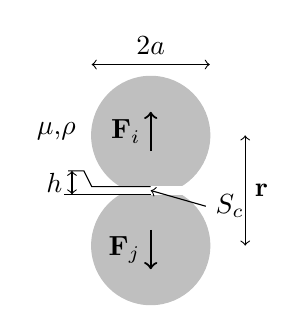
\begin{tikzpicture}
      \draw[lightgray,fill = lightgray] (0,0.7) circle (0.75);
      \draw[lightgray,fill = lightgray] (0,-0.7) circle (0.75);
      \draw[white,fill=white] (-0.75,-0.05) rectangle (0.75,0.05);
      \draw(0,0.05)--++(-0.75,0)--++(-0.1,0.2)--++(-0.2,0);
      \draw(0,-0.05)--++(-1.1,0);
      \draw[<->](-1,-0.05) --++ (0,0.3)node[midway,left]{$h$};
      \draw[<->](-0.75,1.6)--++(1.5,0)node[midway,above]{$2a$};
      \node (para) at (-1.2,0.75){$\mu$,$\rho$};
      \draw[->,thick](0,0.5)--++(0,0.5)node[midway,left]{$\textbf{F}_i$};
      \draw[->,thick](0,-0.5)--++(0,-0.5)node[midway,left]{$\textbf{F}_j$};
      % \draw[<-,thick](1,0.5)--++(0,0.5)node[midway,right]{$\textbf{u}_1$};
      % \draw[<-,thick](1,-0.5)--++(0,-0.5)node[midway,right]{$\textbf{u}_2$};
      \draw[->](0.7,-0.2)node[right]{$S_c$} -- (0,0);
      \draw[<->](1.2,0.7) --++ (0,-1.4) node[right,midway]{$\textbf{r}$} ;
    \end{tikzpicture}
    \caption{Scheme of two colliding droplets labeled $i$ and $j$.}
  \end{figure}
  \column{0.7\textwidth} 
  
  Capillary driven interaction force may be written : 
  \begin{equation*}
    \textbf{f}_{ij}^\text{c}
    = S_c p_\text{Laplace}
    = \pi (a^2 - r_{ij}^2/4) \kappa \gamma  \textbf{r}_{ij}/r_{ij}
\end{equation*} 


For elastic contact only the  particle-particle stress\footnote{It is the stress related to the particle-particle contact force} tensor matter \citep{zhang1997momentum,jackson1997locally} : 
  \begin{align}    
    \pavg{\textbf{f}_i^c}
    &= \frac{1}{2}\div \bm\Sigma_c
\end{align}
% with, 
\begin{equation*}
  \bm\Sigma_c 
  % = \int \sum_{i} \sum_{j \neq i} \delta(\textbf{x}-\textbf{x}_i) (\textbf{x}_{j} - \textbf{x}_i)
  % \textbf{f}_{ij}^c d\PP \\
  =n_p(\textbf{x}) \int_{|\textbf{x}_1 - \textbf{x}| = 2a}
  (\textbf{x} - \textbf{x}_1) \textbf{f}^c(\textbf{x}| \textbf{x}^1) P(\textbf{x}_1|\textbf{x}) d\textbf{x}_1
\end{equation*}

\begin{itemize}
  \item $\gamma$ Surface tension coefficient.  
  \item $\textbf{f}^c(\textbf{x}| \textbf{x}^1)$ mean particle contact force in $\textbf{x}$ knowing a particle is in $\textbf{x}_1$. 
\end{itemize}
\end{columns}


\end{frame}

\begin{frame}
  \frametitle{How to describe pair interactions and microstructure ?}
  % To better model the film drainage problem we need a clear understanding of How the interactions between droplets works. 
  
  \textbf{The nearest particle statistics (Zhang JFM 2020): }
  \begin{definition}
    \begin{itemize}
      \item Let $\mathscr{C} =\left\{\textbf{x}_1, \textbf{r}, \textbf{w},a\right\}$ be the vector containing the position of a particle $\textbf{x}_1$, its nearest neighboring particle relative position $\textbf{r}$, the relative velocity \textbf{w} and the age of the pair time interaction $a$.
      \item Then, $P_{nst}(\textbf{x},\textbf{r},\textbf{w},a) $ is the probability of finding a particle at \textbf{x} with its nearest neighboring particle at \textbf{r} with a relative velocity of \textbf{w} and an age $a$. 
    \end{itemize}
  \end{definition}
  \begin{align*}
    P_{nst}(\textbf{x},\textbf{r},\textbf{w},a)
    &= \int \Pi(\textbf{x},\textbf{r},\textbf{w},a) d\CC\\
    \nstavg{\textbf{f}} P_{nst}(\textbf{x},\textbf{r},\textbf{w},a)
    &= \int \textbf{f} \Pi(\textbf{x},\textbf{r},\textbf{w},a) d\CC
  \end{align*}
  \footnotesize
  \begin{itemize}
    \item 
    where $\Pi = 1$ if and only if a particle is present at \textbf{x} with its nearest neighbor at \textbf{r} = $\textbf{y}-\textbf{x}$, having an age of $a$ with relative velocity \textbf{w}. 
    \item $\textbf{f}$ can be a particle property as well as an Eulerian property of the continuous phase. 
    \item In the following $\textbf{f}$ is either the relative velocity or resultant of force between the particle at \textbf{x} and its nearest neighboring particles at \textbf{y}. 
  \end{itemize}
\end{frame}

\begin{frame}
  \frametitle{Pair probability density function and contact force form DNS Results}

\begin{figure}
  % \includegraphics[height=0.3\textwidth]{image/HOMOGENEOUS_NEW/Capilary_force.png}
  \includegraphics[height=0.3\textwidth]{image/HOMOGENEOUS_NEW/Dist/Pnst_l_10_Ga_100_PHI_0_01.pdf}
  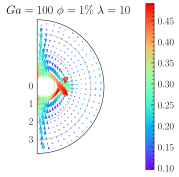
\includegraphics[height=0.3\textwidth]{image/HOMOGENEOUS_NEW/Dist/U_rel_l_10_Ga_100_PHI_1.pdf}
  \includegraphics[height=0.3\textwidth]{image/HOMOGENEOUS_NEW/Dist/F_rel_l_10_Ga_100_PHI_1.pdf}
  \caption{DNS results (left) Pair probability density function $P_\text{nst}(\textbf{r})$. 
  (center) Conditionally averaged relative velocity. Color map : age of the interaction, Made dimensionless with the inertial time scale : $\sqrt{diameter/gravity}$.  
  (right) Conditionally averaged relative total force $\textbf{f} = \int_\Sigma \bm\sigma_1^0\cdot \textbf{n}_2 d\Sigma$. Made dimensionless with the capillary scale $a\sigma$.  
  }
\end{figure}

\begin{enumerate}
  \item[Remark 1.]The pair PDF is not exactly isotropic (= more particle above than on the sides). 
  \item[Remark 2.] The relative velocity show that :
  Particles come from the vertical and leave through the side. 
  \item[Remark 3.] The resultant of the  force  on the particles is largely dominated by the capillary forces.
\end{enumerate}

\end{frame}
\begin{frame}
  \frametitle{Weighted pair probability density function and contact force form DNS Results}

\begin{figure}
  % \includegraphics[height=0.3\textwidth]{image/HOMOGENEOUS_NEW/Capilary_force.png}
  \includegraphics[height=0.3\textwidth]{image/HOMOGENEOUS_NEW/Dist/Pnst_l_10_Ga_100_PHI_0_01.pdf}
  \includegraphics[height=0.3\textwidth]{image/HOMOGENEOUS_NEW/Dist/UW_rel_l_10_Ga_100_PHI_1.pdf}
  \includegraphics[height=0.3\textwidth]{image/HOMOGENEOUS_NEW/Dist/FW_rel_l_10_Ga_100_PHI_1.pdf}
  \caption{DNS results (left) Pair probability density function $P_\text{nst}(\textbf{r})$. 
  (right) Conditionally weighted averaged relative velocity. Color map : age of interaction. 
  (right) Conditionally averaged  weighted relative total force $P_\text{nst}\textbf{f} = hydro+contact$. Made dimensionless with the capillary scale $a\sigma$.  
  }
\end{figure}

\begin{enumerate}
  \item[Remark 1.]The pair PDF is not exactly isotropic (= more particle above than on the sides). 
  \item[Remark 2.] The relative velocity show that :
  Particles come from the vertical and leave through the side. 
  \item[Remark 3.] The resultant of the  force  on the particles is largely dominated by the capillary forces.
\end{enumerate}

\end{frame}

\begin{frame}
  \frametitle{Comparison of the force with the present model. }
  \begin{columns}
    \column{0.3\textwidth}
    The most simple model : 
  
    \begin{equation*}
      \textbf{f}_{ij}^\text{c}
      = \pi (a^2 - r_{ij}^2/4) \kappa \gamma  \textbf{r}_{ij}/r_{ij}
    \end{equation*} 
    Or in average : 
    \begin{equation}
      \textbf{f}^c(\textbf{x}| \textbf{x}_1)
      = \pi (a^2 - \textbf{r}\cdot\textbf{r}/4) \kappa \gamma 
      \frac{\textbf{r}}{r}
      \label{eq:fcond}
    \end{equation} 
    The particle-particle contact force stress can be obtained form : 
    \begin{equation*}
      \bm\Sigma_c 
      =\int_{|\textbf{x}_1 - \textbf{x}| = 2a}
      \textbf{r} \textbf{f}^c(\textbf{r}) P(\textbf{r}) d\textbf{}
    \end{equation*}

    \column{0.7\textwidth}

    \begin{figure}
      % \includegraphics[height=0.3\textwidth]{image/HOMOGENEOUS_NEW/Capilary_force.png}
      \includegraphics[height=0.4\textwidth]{image/HOMOGENEOUS_NEW/Capilary_force_l_1_Ga_10.pdf}
      \includegraphics[height=0.4\textwidth]{image/HOMOGENEOUS_NEW/Capilary_force_l_1_Ga_100.pdf}
      \caption{Radial averaged value of the relative total force between particles $\textbf{f}(\textbf{r}) = hydro+contact$, in terms of the particles distances \textbf{r}.
      (black dashed lines) Model form Equation \ref{eq:fcond}. 
      (grey dot dashed lines) Pressure contribution to the total force from DNS. 
      ($\blacktriangle$) $\phi = 20$\% 
      ($\bullet$) $\phi = 1$\%} 
    \end{figure}

  \end{columns}


\end{frame}

\begin{frame}[t]
  \frametitle{References}
  \bibliography{Bib/bib_bulles.bib}
\end{frame}

\end{document}
